\nomenclature[940]{ghc\dotfill}{The Glasgow Haskell Compiler}
\nomenclature[941]{JSON\dotfill}{JavaScript Object Notation}

\chapter{Implementation\index{Implementation}}
\label{chp:implementation}
In this chapter, we describe two implementations\index{Implementation} of the calculus from \chpref{chp:algebraic_model} in \textsf{Haskell}\index{Haskell}. We design our implementation in \textsf{Haskell} to closely resemble the structure and semantics of our calculus, so it is straightforward to transform process structures formulated in \textsf{Haskell} into a representation in our calculus and reason about them. As a useful consequence, the laws stated in \chpref{chp:laws} transform from the calculus to processes in our implementation and remain valid.

For one of the implementations, we use \textsf{Concurrent Haskell}\index{Concurrent Haskell}\index{Haskell!Concurrent Haskell} and fork local threads in the \texttt{IO} monad for parallelisation on one computer. For the other one, we use \textsf{Cloud Haskell}\index{Cloud Haskell}\index{Haskell!Cloud Haskell} to distribute processes into a distributed system and run them in \textsf{Cloud Haskell}'s \texttt{Process} monad. Other implementations based on, e.g. \textsf{Parallel Haskell} are imaginable.

Ideally, we want the two implementations to be usable interchangeably by simply importing the desired implementation and without changing any of the productive code, however, we cannot achieve this at the moment. When using the implementation based on \textsf{Cloud Haskell}, we need to require additional properties of the data types that are transmitted over the network to other processes. Furthermore, in order to run code remotely, the code has to be known on the remote node since \textsf{ghc}\footnote{The Glasgow Haskell Compiler, c.f. \url{https://www.haskell.org/ghc/}.}\index{GHC} does not support serialising and transmitting functions over the network \cite{Epstein:2011:THC:2034675.2034690}. To solve this problem, a trick is used that requires us to change the model of basic processes slightly. However, we are optimistic that in future versions of \textsf{ghc}, it will be possible to achieve full interchangeability of both (and possibly more) implementations.


\clearpage

\section{Implementation using Concurrent Haskell\index{Concurrent Haskell}\index{Haskell!Concurrent Haskell}}
\label{chp:local}
In the implementation for local parallelisation on one computer, we make use of \textsf{Concurrent Haskell}\index{Concurrent Haskell}\index{Haskell!Concurrent Haskell}. Basic processes are represented as computations in the \texttt{IO} monad. Parallelisation is achieved by running processes that are modelled for parallel execution concurrently in lightweight threads using \texttt{forkIO}, synchronisation is done using \texttt{MVar}s.

An introduction to \textsf{Concurrent Haskell} and \textsf{Haskell}'s \texttt{IO} monad can be found in standard \textsf{Haskell} literature such as \cite{Hutton}, \cite{Bird} or \cite{Marlow}. The fact that we use the \texttt{IO} monad has immediate consequences: we cannot force processes to be free of side-effects\index{Side-effect}, hence they can perform actions like, e.g. reading from or writing to the file system.

\subsection{Data model\index{Data Model}}
\label{chp:local_model}
Our data model directly resembles the structure of the syntactic rules of process composition from \chpref{chp:syntax}. We use the power of \textsf{Haskell}'s type system and a generalised algebraic data type\index{Generalised Algebraic Data Type} to assure the model meets the requirements concerning static semantics formulated in \chpref{chp:static_semantics} and prevent the creation of invalid processes with respect to static semantics.

As mention before, basic processes are computations in the \texttt{IO} monad. They receive an input of type \texttt{a} and output a value of type \texttt{b}.
\begin{lstlisting}[language=Haskell,caption=Representation of basic processes as computations in the \texttt{IO} monad.,label=fig:local_computation,numbers=left,frame=bt]
type BasicProcess a b = a -> IO b
\end{lstlisting}

Predicates\index{Predicate} are represented as processes that receive an input and output a value of type \texttt{Bool}, as introduced in \chpref{chp:static_semantics}.
\begin{lstlisting}[language=Haskell,caption=Representation of predicates as processes.,label=fig:local_computation,numbers=left,frame=bt,firstnumber=2]
type Predicate a = Process a Bool
\end{lstlisting}

The data type for processes involves two type parameters\index{Type!Parameter}, \texttt{a} and \texttt{b}. They reflect the process' input and output types where \texttt{a} is the input type and \texttt{b} is the output type.
\begin{lstlisting}[language=Haskell,caption=Data type for the representation of processes.,label=fig:local_datatypes,numbers=left,frame=bt,firstnumber=3]
data Process a b where
\end{lstlisting}

The identity process and the error process are modelled using the \texttt{Id}\index{Data constructor!Id} and the \texttt{Err}\index{Data constructor!Err} data constructors. Their type signatures are as stated in \defref{def:static_id_err}.
\begin{lstlisting}[language=Haskell,caption=Signatures of the \texttt{Id} and \texttt{Err} data constructors.,label=fig:local_datatypes,numbers=left,frame=bt,firstnumber=4]
Id  :: Process a a
Err :: Process a a
\end{lstlisting}

Basic processes are turned into processes by wrapping them using the \texttt{Basic}\index{Data constructor!Basic} data constructor. The developer is cautioned about using basic processes that incorporate side-effects as they potentially render the laws given in \chpref{chp:laws} invalid. \texttt{Basic}\index{Data constructor!Basic} takes a basic process\index{Process!Basic} of type \texttt{BasicProcess a b}, i.e. a computation in the \texttt{IO} monad that takes an input of type \texttt{a} and outputs a value of type \texttt{b}, and creates a process from it.
\begin{lstlisting}[language=Haskell,caption=Signature of the \texttt{Basic} data constructor.,numbers=left,frame=bt,firstnumber=6]
Basic :: BasicProcess a b
      -> Process a b
\end{lstlisting}

The \texttt{Choice}\index{Data constructor!Choice} data constructor is used to build a process that makes a choice between two processes. Its type signature satisfies \defref{def:static_choice}: \texttt{Choice} takes a predicate of type \texttt{Predicate a}, two processes of type \texttt{Process a b} and results in a process of type \texttt{Process a b}.
\begin{lstlisting}[language=Haskell,caption=Signature of the \texttt{Choice} data constructor.,numbers=left,frame=bt,firstnumber=8]
Choice :: Predicate a
       -> Process a b
       -> Process a b
       -> Process a b
\end{lstlisting}

The \texttt{Parallel}\index{Data constructor!Parallel} data constructor is used to model parallel composition of processes, its type signature reflects \defref{def:static_parallel}. It takes two processes for parallel composition with type signatures \texttt{Process a c} and \texttt{Process a d} as well as a third process of type \texttt{Process (c, d) b} that is used to combine the results of the other two processes.
\begin{lstlisting}[language=Haskell,caption=Signature of the \texttt{Parallel} data constructor.,numbers=left,frame=bt,firstnumber=12]
Parallel :: Process (c, d) b
         -> Process a c
         -> Process a d
         -> Process a b
\end{lstlisting}

The \texttt{Sequence}\index{Data constructor!Sequence} data constructor takes two processes for sequential composition. Just as for conventional function composition, the output type of the first process and the input type of the second process must coincide, as stated in \defref{def:static_sequence}.
\begin{lstlisting}[language=Haskell,caption=Signature of the \texttt{Seqeuence} data constructor.,numbers=left,frame=bt,firstnumber=16]
Sequence :: Process a c
         -> Process c b
         -> Process a b
\end{lstlisting}

With the \texttt{Repetition}\index{Data constructor!Repetition} data constructor, a process can be wrapped for repeated execution. \texttt{Repetition} takes a predicate of type \texttt{Predicate a} and a process of type \texttt{Process a a}, as defined in \defref{def:static_repetition}.
\begin{lstlisting}[language=Haskell,caption=Signature of the \texttt{Repetition} data constructor.,numbers=left,frame=bt,firstnumber=19]
Repetition :: Predicate a
           -> Process a a
           -> Process a a
\end{lstlisting}

In addition to the combinators introduced in \chpref{chp:syntax}, the implementation contains the \texttt{Multilel} combinator. \texttt{Multilel}\index{Data constructor!Multilel} provides a convenient short-hand notation for the parallel composition of a list of processes instead of exactly two as is the case for the \texttt{Parallel} combinator. It takes a list of processes of type \texttt{Process a c} and a process of type \texttt{Process (a, [c]) b}. The list of processes contains the processes that should be composed in parallel, the additional process is used to combine the results of the processes together into one value. \texttt{Multilel} does not change the expressiveness of the model, in fact it can be expressed in terms of parallel and sequential composition.
\begin{lstlisting}[language=Haskell,caption=Signature of the \texttt{Multilel} data constructor.,numbers=left,frame=bt,firstnumber=22]
Multilel :: [Process a c]
         -> Process (a, [c]) b
         -> Process a b
\end{lstlisting}

\subsection{Process interpreter\index{Process Interpreter}}
In this section, we discuss how the Process interpreter works in detail by taking a look at its implementation.

Processes can be executed by providing them with an input using the \texttt{runProcess} function. \texttt{runProcess} runs in the \texttt{IO} monad, it takes a process of type \texttt{Process a b} and an input for that process of matching type. The execution of a process yields a result of type \texttt{b}. \texttt{runProcess} is the implementation of the function $sem$ introduced in \chpref{chp:semantics} that defines the semantics of processes.
\begin{lstlisting}[language=Haskell,caption=Signature of the process interpreter implemented using \textsf{Concurrent Haskell}.,label=lst:local_runprocess_signature,numbers=left,frame=bt]
runProcess :: Process a b -> a -> IO b
\end{lstlisting}

The semantics of an \texttt{Id}\index{Process Interpreter!Id} process is as given in \defref{def:sem_id}: it simply outputs its input.
\begin{lstlisting}[language=Haskell,caption=Implementation of the interpreter for \texttt{Id} processes.,label=lst:local_runprocess_const,numbers=left,frame=bt,firstnumber=2]
runProcess Id x =
  return x
\end{lstlisting}

The semantics of an \texttt{Err}\index{Process Interpreter!Err} process is as stated in \defref{def:sem_err}. The error process outputs the undefined value regardless of its input.
\begin{lstlisting}[language=Haskell,caption=Implementation of the interpreter for \texttt{Err} processes.,label=lst:local_runprocess_const,numbers=left,frame=bt,firstnumber=4]
runProcess Err _ =
  return undefined
\end{lstlisting}

A \texttt{Basic}\index{Process Interpreter!Basic} process is simply a wrapper for a computation \texttt{f} in the \texttt{IO} monad, which is the equivalent of an intrinsic function\index{Intrinsic Function} of a basic process as described in \chpref{chp:semantics}. The interpretation of a \texttt{Basic} process is done by applying the process's intrinsic function \texttt{f} to the process's input \texttt{x}, as given in \defref{def:sem_atomic}.
\begin{lstlisting}[language=Haskell,caption=Implementation of the interpreter for \texttt{Basic} processes.,label=lst:local_runprocess_simple,numbers=left,frame=bt,firstnumber=6]
runProcess (Basic f) x =
  f x
\end{lstlisting}

For the interpretation of \texttt{Choice} processes, the output of \texttt{predicate}, when supplied with input \texttt{x}, has to be obtained first by making use of the interpreter function \texttt{runProcess}. Then, based on the predicate's output, the choice between executing either \texttt{p1} or \texttt{p2} is made as defined in \defref{def:sem_choice}.
\index{Process Interpreter!Choice}
\begin{lstlisting}[language=Haskell,caption=Implementation of the interpreter for \texttt{Choice} processes.,label=lst:local_runprocess_choice,numbers=left,frame=bt,firstnumber=8]
runProcess (Choice predicate p1 p2) x = do
  b <- runProcess predicate x
  runProcess (if b then p1 else p2) x
\end{lstlisting}

A \texttt{Parallel}\index{Process Interpreter!Parallel} process involves two process for concurrent execution, namely \texttt{p1} and \texttt{p2}, as well as a combinator process \texttt{combinator} to combine the outputs of \texttt{p1} and \texttt{p2}. In order to execute two processes at the same time, a second thread needs to be forked and the interpretation of one of the processes has to be done there. To do so, the auxiliary function \texttt{runProcessHelper} is implemented: \texttt{runProcessHelper} takes a process \texttt{p} that should be interpreted, an input \texttt{x} for \texttt{p} and an \texttt{MVar}. \texttt{runProcessHelper} determines the output of \texttt{p}, applied to \texttt{x}, by making use of \texttt{runProcess} and saves the output to the \texttt{MVar}.
\begin{lstlisting}[language=Haskell,caption=Auxiliary function for the interpretation of \texttt{Parallel} processes.,label=lst:local_runprocesshelper,numbers=left,frame=bt,firstnumber=11]
runProcessHelper :: Process a b -> a -> MVar b -> IO ()
runProcessHelper p x mvar = putMVar mvar =<< runProcess p x
\end{lstlisting}

To interpret a \texttt{Parallel} process, an empty \texttt{MVar} is created and, together with \texttt{p1} and input \texttt{x}, passed on to \texttt{runProcessHelper} that is forked in a new thread using \texttt{forkIO}. While the output of \texttt{p1} is determined in the new thread, the interpreter determines the output of \texttt{p2} in its local thread. The previously created \texttt{MVar} is used to comfortably wait for the output of \texttt{p1} that \texttt{runProcessHelper} saves to the \texttt{MVar} once it has been obtained. Finally, \texttt{combinator} is used to combine the outputs of \texttt{p1} and \texttt{p2} into a single value, as given in \defref{def:sem_parallel}.
\begin{lstlisting}[language=Haskell,caption=Implementation of the interpreter for \texttt{Parallel} processes.,numbers=left,frame=bt,label=lst:local_runprocess_parallel,firstnumber=13]
runProcess (Parallel p1 p2 combinator) x = do
  mvar <- newEmptyMVar
  _    <- forkIO $ runProcessHelper p1 x mvar
  r2   <- runProcess p2 x
  r1   <- takeMVar mvar
  runProcess combinator (r1, r2)
\end{lstlisting}

For the interpretation of a \texttt{Sequence}\index{Process Interpreter!Sequence} process, \texttt{runProcess} is employed to obtain the output of \texttt{p1} when supplied with input \texttt{x}. Then, the output of \texttt{p1} if used as input for the interpretation of \texttt{p2} with \texttt{runProcess}, as defined in \defref{def:sem_sequence}. The implementation of this is straightforward, using the bind operator \texttt{>}\texttt{>=}.
\begin{lstlisting}[language=Haskell,caption=Implementation of the interpreter for \texttt{Sequence} processes.,label=lst:local_runprocess_sequence,numbers=left,frame=bt,firstnumber=19]
runProcess (Sequence p1 p2) x =
  runProcess p1 x >>= runProcess p2
\end{lstlisting}

The \texttt{Repetition}\index{Process Interpreter!Repetition} process is used to express repeated execution of a process. As stated in \defref{def:sem_repetition}, repetition is expressed in terms of a combination of choice and sequential composition.
\begin{lstlisting}[language=Haskell,caption=Implementation of the interpreter for \texttt{Repetition} processes.,numbers=left,frame=bt,firstnumber=21]
runProcess rep@(Repetition predicate p) x =
  runProcess (Choice predicate (p `Sequence` rep) Id) x
\end{lstlisting}

Finally, there is the \texttt{Multilel}\index{Process Interpreter!Multilel} process that can be expressed as a combination of \texttt{Parallel} and \texttt{Sequence} processes. The list of processes that should all be executed in parallel is transformed into a hierarchy of parallel processes, composed using the \texttt{Parallel} data constructor, by \texttt{foldr}. For the combination of the processes' results, two helper processes are employed: \texttt{emptyListP} and \texttt{consP}. \texttt{emptyListP} is a process that ignores its input and returns the empty list. \texttt{consP} is the process variant of the cons operator \texttt{(:)} and is used together with \texttt{emptyListP} to produce the list of result values. A third helper process \texttt{pairP} is used to create a pair of the original input value \texttt{x} and the list of result values from the parallel composition of processes. The final result of the \texttt{Multilel} process is produced by folding the result values together using the process \texttt{fold}.
\begin{lstlisting}[language=Haskell,caption=Implementation of the interpreter for \texttt{Multilel} processes.,label=lst:local_runprocess_multilel,numbers=left,frame=bt,firstnumber=23]
runProcess (Multilel ps fold) x =
  flip runProcess x $
               foldr (Parallel consP) emptyListP ps 
    `Sequence` pairP x
    `Sequence` fold
  where
    -- a process that creates a pair with first component x
    -- and second component given by its input
    pairP :: a -> Process b (a, b)
    pairP x = Basic (\y -> return (x,y))
 
    -- process variant of the cons operator on lists
    consP :: Process (c, [c]) [c]
    consP = Basic (return . uncurry (:))

    -- a process that ignores its input and returns the empty list
    emptyListP :: Process a [c]
    emptyListP = Basic (return . const [])
\end{lstlisting}


\clearpage

\section{Implementation using Cloud Haskell\index{Cloud Haskell}\index{Haskell!Cloud Haskell}}
\label{chp:distributed}
In the implementation for distributed parallelisation of process interpretation, we use \textsf{Cloud Haskell} and execute processes in \textsf{Cloud Haskell}'s \texttt{Process} monad. The involvement of network communication requires instances of specific type classes for the types that are sent to other processes. Furthermore, the representation of basic processes needs to be adapted to the specifics of \textsf{Cloud Haskell}. 

\subsection{Cloud Haskell\index{Cloud Haskell}\index{Haskell!Cloud Haskell}}
\label{chp:cloud_haskell}
\textsf{Cloud Haskell} \cite{Epstein:2011:THC:2034675.2034690} is a domain specific language for distributed programming in \textsf{Haskell}\index{Haskell}. It is highly inspired by \textsf{Erlang}\index{Erlang} and its message passing\index{Message passing} mechanism for communication between processes, with no implicit shared memory involved.

A \textsf{Cloud Haskell} process is essentially a function\index{Function} that is evaluated in the \textsf{Cloud Haskell} \texttt{Process} monad and can be spawned on a local\index{Node!Local} or remote\index{Node!Remote} node. Processes can send messages to other processes if they have knowledge about their process identifier, which serves as an address. The \texttt{Process} monad builds on top of the \texttt{IO} monad and thus, as mentioned in \chpref{chp:local}, we cannot force processes to be free of side-effects.

While \textsf{Erlang}\index{Erlang} uses atoms as tags for messages, \textsf{Cloud Haskell} uses data types that need to have an instance of \texttt{Serializable}. \texttt{Serializable} itself is only a combination of both \texttt{Binary} and \texttt{Typeable}. \texttt{Binary} is neccessary to serialise a message into a \texttt{ByteString}, \texttt{Typeable} is used to identify the type of a value. This way, serialisation\index{Serialisation} is made explicit, in contrast to \textsf{Erlang} where it is implicit \cite{Epstein:2011:THC:2034675.2034690}.

In \textsf{Haskell}, functions can only be executed, composed and passed as arguments, they cannot be serialised. However, this is necessary in order to send a function to a remote\index{Node!Remote} node and execute it there. \textsf{Cloud Haskell} avoids this problem by using fully qualified top level names of functions that are known at compile time in a table of static code pointers to refer to functions by their name. For remote execution, a function's name is put into a closure\index{Closure}, together with its serialised environment\index{Environment}, i.e. its argument, and sent to a remote node where it is deserialised and executed. A closure is a function (name) together with its argument \cite{Epstein:2011:THC:2034675.2034690} and can be created using \textsf{Cloud Haskell}'s function \texttt{mkClosure} and \textsf{Template Haskell}\footnote{The function that should be executed remotely is actually combined with a matching decoder for its input.}. \texttt{mkClosure} takes the top level name of a 1-ary function of some type \texttt{a \nolinebreak $\to$ Process b} and returns a process closure generator. For a function \texttt{f} with type \texttt{a \nolinebreak $\to$ \nolinebreak Process b}, the type of \texttt{\$(mkClosure 'f)} resolves to \texttt{a \nolinebreak $\to$ Closure (Process b)}, i.e. it is a closure generator that generates a closure when supplied with a value of type \texttt{a}.

After a closure has been executed, the result is serialised and sent back to the caller. However, the type system cannot infer the type and serialisability of the result automatically and therefore additional information needs to be provided\footnote{Specifically, the problem is that the type constructors can be constrained with required type class instances for parameters. On deconstruction, this information is not available and therefore needs to be added explicitly again.}. For a type \texttt{a}, serialisation information can be provided with a value of type \texttt{Static (SerializableDict a)}. Basically, this is an explicit type tag that enables the selection of the correct serialisation function for type \texttt{a}.

\subsection{Data model\index{Data Model}}
\label{chp:distributed_model}
The data model for the representation of processes stays almost unchanged: only the definition of basic processes and the \texttt{Basic} data constructor for processes have to be adapted to meet specific requirements that arise with the use of \textsf{Cloud Haskell}. Basic processes are now functions that take an input of type \texttt{a} and return a closure that contains a \textsf{Cloud Haskell} process producing an output of type \texttt{b} when executed.
\begin{lstlisting}[language=Haskell,caption=Representation of basic processes as computations in the \texttt{CH.Process} monad.,numbers=left,frame=bt]
import qualified Control.Distributed.Process as CH

type BasicProcess a b = a -> CH.Closure (CH.Process b)
\end{lstlisting}

The form of the data type for the representation of processes remains unchanged.
\begin{lstlisting}[language=Haskell,caption=Data type for the representation of processes.,label=lst:distributed_datatypes,numbers=left,frame=bt,firstnumber=4]
data Process a b where
\end{lstlisting}

\texttt{Basic}\index{Data constructor!Basic} reflects the adaptations that are necessary to use \textsf{Cloud Haskell} for remote interpretation of processes: the output type of the wrapped basic process must have an instance of \texttt{Serializable} and a static \texttt{SerializableDict} for the same type must be provided. As mentioned in \chpref{chp:cloud_haskell}, this is necessary so remotely\footnote{This is true for locally spawned processes as well, as we cannot distinguish between them: \textsf{Cloud Haskell} transparently takes care of that we can use both local and remote processes in the same way. Technically, however, we could inspect the process identifier and tell whether the respective process is running on the local node or not.} spawned processes know how to serialise their output and send it back to the caller.
\begin{lstlisting}[language=Haskell,caption=Signature of the \texttt{Basic} data constructor.,numbers=left,frame=bt,firstnumber=5]
Basic :: (Serializable b)
      => CH.Static (SerializableDict b)
      -> BasicProcess a b
      -> Process a b
\end{lstlisting}

A new processes type, \texttt{Local}\index{Data constructor!Local}, is added to the model. \texttt{Local} is a simple decorator\index{Decorator} \cite{Gamma:1995:DPE:186897}, with the purpose of giving an indication to the process interpreter that the wrapped process should be executed locally. Typically, the reason for this arises from the expectation that serialising a closure, sending it to a remote node, executing it there and obtaining the result is more expensive\footnote{Expensive in terms of the necessary amount of time to run the process.} than executing the respective process locally. Since there is no general approach to estimate the necessary amount of time to run a process, the decision has been made to equip the developer with a tool to force local execution of a process and burden him with the obligation to make appropriate use of it.
\begin{lstlisting}[language=Haskell,caption=Signature of the additional \texttt{Local} data constructor.,numbers=left,frame=bt,firstnumber=9]
Local :: Process a b
      -> Process a b
\end{lstlisting}

The signatures of the rest of the data constructors, i.e. \texttt{Parallel}\index{Data constructor!Parallel}, \texttt{Sequence}\index{Data constructor!Sequence}, \texttt{Repetition}\index{Data constructor!Repetition} and \texttt{Multilel}\index{Data constructor!Multilel}, remain unchanged.

\subsection{Architecture of the distribution infrastructure\index{Architecture}\index{Infrastructure}}
\label{chp:infrastructure}
For the interpretation of process structures in a distributed system, some kind of infrastructure and management of involved nodes is needed, so process execution can be delegated to them. In this section, we describe the architecture and functioning of our system.
\vspace*{-0.5em}
\begin{figure}[h!]
  \centering
  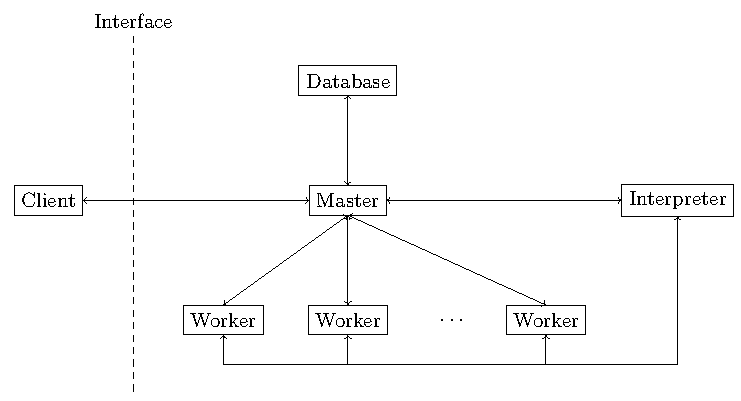
\includegraphics[width=\textwidth]{img/architecture.pdf}
  \caption{Architecture of the distribution infrastructure.}
  \vspace*{-0.5em}
  \label{fig:architecture}
\end{figure}

The architecture of the system's infrastructure is intentionally kept simple and is as shown in \figref{fig:architecture}. It involves a designated \textbf{master}\index{Node!Master} node and a collection of \textbf{worker}\index{Node!Worker} nodes. The master node provides an interface\index{Interface} through which processes can be inserted into the system by a client.

When a client\index{Client} wants to submit a request\index{Request}, he has to make use of the interface and supply a problem description in an appropriate format, e.g. a JSON\footnote{JavaScript Object Notation, see \url{http://www.json.org/}}\index{JSON} document. A parser reads the submitted JSON document, generates a corresponding process structure from its content and passes it on to the process interpreter if the document contains a valid process description. For simplicity, we assume in the following that a request equals an interpretable process description.

The master\index{Node!Master} node is responsible for handling client\index{Client} requests, logging information related to the received requests and managing connected nodes. When a request is received, the master spawns a new \textsf{Cloud Haskell} process that runs the process interpreter\index{Interpreter} and passes the request to the new process where it is interpreted. At the same time, the master assigns a ticket ID to the request, logs the request together with its ID to a database\footnote{For this purpose, the \texttt{acid-state} library is used. \texttt{acid-state} allows to save \textsf{Haskell} values into a file-based database if their type has an instance of \texttt{SafeCopy}. Further information on \texttt{acid-state} can be found at \url{http://acid-state.seize.it/} and \url{https://github.com/acid-state/acid-state}} and reports the ticket ID to the client. When the interpreter finishes interpretation of the process structure from the request, it reports the result to the master. The master saves the result to the database and associates it with the according ticket ID. At any time, the client can try to retrieve the result by supplying the request's ticket ID to the master through the interface. The master then tries to read the result from the database, but only replies to the client's satisfaction after the interpretation of the request has been finished and the result logged to the database.

Worker nodes\index{Node!Worker} are kept very simple. When started and supplied with the master's address, i.e. its process identifier, they report their availability to the master and wait for further instruction.

The process interpreter\index{Interpreter} is run in a new process by the master for every client request\index{Request} that is received. The interpreter takes the process description from the request and distributes the incorporated sub-processes\index{Sub-process} to worker\index{Node!Worker} nodes or executes them locally if they have been marked for local execution using the \texttt{Local} wrapper. For every basic process, the interpreter asks the master for a worker node on which it can run the basic process. When receiving a request for a worker node, the master fetches a worker node from a FIFO queue and returns it to the interpreter as soon as there is one available. After a basic process has finished execution on a worker node, the interpreter returns the respective worker node to the master for future allocation to other interpreters.

The source code of the distribution system can be found in \appref{app:dvd}.


\subsection{Process interpreter\index{Process Interpreter}\index{Interpreter}}
\label{chp:interpreter}
Now that a distributed system is involved, the implementation of the process interpreter needs to be adapted to this situation. Where there was only local parallelisation in the \texttt{IO} monad in \textsf{Concurrent Haskell} involved before, process interpretation has to be adapted to the specifics of the \textsf{Cloud Haskell}\index{Cloud Haskell} \texttt{Process} monad. This particularly involves execution of processes on remote nodes.

When the master\index{Node!Master} node receives a client\index{Client} request\index{Request}, it spawns a process interpreter on its local node and passes the process structure from the request to the interpreter. The interpreter then inspects the process structure and distributes the incorporated sub-processes\index{Sub-process} to connected worker nodes accordingly. To do so, the interpreter asks the master node for an available worker node for every sub-process of the form \texttt{Basic} that has to be executed\footnote{Except for processes wrapped into a \texttt{Local} process, of course.}. The master\index{Node!Master} node is represented by a \texttt{ProcessId}, wrapped into a value of type \texttt{Master}.
\begin{lstlisting}[language=Haskell,caption=Data type for the representation of the address of the master node.,numbers=left,frame=bt]
newtype Master = Master ProcessId
\end{lstlisting}

The signature of \texttt{runProcess} has to be extended by an additional parameter: a value of type \texttt{Master} that carries information about the master node's address.
\begin{lstlisting}[language=Haskell,caption=Signature of the process interpreter implemented using \textsf{Cloud Haskell}.,label=lst:interpreter_signature,numbers=left,frame=bt,firstnumber=2]
runProcess :: Master -> Process a b -> a -> CH.Process b
\end{lstlisting}

For a \texttt{Basic}\index{Process Interpreter!Basic} process in a process structure, the process interpreter asks the master node for an available worker node on which it can run the wrapped basic process. This operation blocks until the master node is able to satisfy the request for an available worker node and supplies it to the interpreter. The interpreter then uses the closure generator \texttt{closureGen} to generate a closure that is serialised and sent to the worker node for execution. This operation blocks until execution of the remotely spawned process has terminated and a result is obtained. The interpreter gives the worker node back to the master and returns the remotely calculated result to its caller.
\begin{lstlisting}[language=Haskell,caption=Implementation of the interpreter for \texttt{Basic} processes.,label=lst:runprocess_simple,numbers=left,frame=bt,firstnumber=3]
runProcess master (Basic sDict closureGen) x = do
  node <- getNode master
  res  <- call sDict node (closureGen x)
  returnNode master node
  return res
\end{lstlisting}

\vspace*{-0.5em}
Processes that are wrapped into a \texttt{Local}\index{Process Interpreter!Local} wrapper are supposed to be executed locally on the same node by the process interpreter instead of being distributed to remote nodes. This includes all sub-processes\index{Sub-process}. To accomplish this behaviour, a little trick is applied: a fake master that always returns the local node when asked for an available worker node is created and used for all sub-processes of the \texttt{Local} process. When interpretation of all sub-process has finished, the fake master is terminated.
\begin{lstlisting}[language=Haskell,caption=Implementation of the interpreter for \texttt{Local} processes.,label=lst:runprocess_local,numbers=left,frame=bt,firstnumber=8]
runProcess _ (Local p) x = do
  fakeMaster <- getFakeMaster
  res <- runProcess fakeMaster p x
  terminateMaster fakeMaster
  return res
\end{lstlisting}

\vspace*{-0.5em}
A problem arises in the interpretation of \texttt{Multilel}\index{Process Interpreter!Multilel} processes. Where it was possible to create auxiliary processes for the representation of \texttt{Multilel} processes in terms of \texttt{Parallel} and \texttt{Sequence} in the implementation based on \textsf{Concurrent Haskell}, this is not possible in \textsf{Cloud Haskell} at the moment. Processes of type \texttt{Basic} require a \textbf{specific} \texttt{SerializableDict} for the type of their output, which must be known at compile time. This prevents the use of polymorphic processes and makes a direct implementation of the parallelisation necessary, analogous to the interpretation of \texttt{Parallel} processes. For each of the processes that should be executed in parallel, \texttt{runProcessHelper} is spawned in a new thread\footnote{Spawning a process in \textsf{Cloud Haskell} is actually implemented using the \texttt{forkIO} functionality from \textsf{Concurrent Haskell} and creates a lightweight thread on a node.}, receiving an \texttt{MVar} to take up the output of the respective process. When all processes have terminated and their outputs have been obtained from the \texttt{MVar}s, the process \texttt{fold} is used to combine the results together into a single value.
\begin{lstlisting}[language=Haskell,caption=Implementation of the interpreter for \texttt{Multilel} processes.,label=lst:runprocess_multilel,numbers=left,frame=bt,firstnumber=13]
runProcess master (Multilel ps fold) x = do
  mvars <- forM ps $ \_ -> liftIO newEmptyMVar
  mapM_ (\(p, m) -> spawnLocal $ runProcessHelper master p x m)   (ps `zip` mvars)
  ress  <- forM mvars $ \mvar -> liftIO . takeMVar $ mvar
  runProcess master fold (x, ress)
\end{lstlisting}

\vspace*{-0.5em}
The adaptations that have to be made for the interpretation of the remaining process types, i.e. \texttt{Choice}\index{Process Interpreter!Choice}, \texttt{Parallel}\index{Process Interpreter!Parallel}, \texttt{Sequence}\index{Process Interpreter!Sequence} and \texttt{Repetition}\index{Process Interpreter!Repetition} are minimal. They involve adding the necessary \texttt{master} parameter and adaptations specific to the \textsf{Cloud Haskell} \texttt{Process} monad, i.e. using \texttt{spawnLocal} instead of \texttt{forkIO} and lifting actions on \texttt{MVar}s into the \textsf{Cloud Haskell} \texttt{Process} monad using \texttt{liftIO}. The implementation can be found in \appref{app:distributed_split_slice} and \appref{app:dvd}.


\clearpage
\section{Example: a parallel interpreter for arithmetic expressions\index{Example}}
\label{chp:example}
After discussing the process model and the interpreter that takes care of process interpretation, we give an example of how to apply the process calculus. To do so, we develop the typical hello world program for interpreters, i.e. an interpreter\index{Interpreter} for arithmetic expressions\index{Arithmetic Expression} with parallel evaluation of sub-expressions. Except for the import of our process calculus, this example is self-contained and is intentionally kept very simple. The necessity of a parallelised interpreter for arithmetic expressions is certainly not given. However, an interpreter for arithmetic expressions is fairly simple and thus well suited to illustrate how to apply the process calculus to it.

An arithmetic expression \texttt{Expr} is either a value \texttt{Val} containing an \texttt{Int} or a combination of two arithmetic expressions. The combinators for arithmetic expressions are addition \texttt{Add}, subtraction \texttt{Sub}, multiplication \texttt{Mul} and division \texttt{Div}.
\begin{lstlisting}[language=Haskell, caption=Data model for the representation of arithmetic expressions., label=lst:arith_model, numbers=left, frame=bt]
data Expr = Val Int
          | Add Expr Expr
          | Sub Expr Expr
          | Mul Expr Expr
          | Div Expr Expr
\end{lstlisting}

The semantics of an \texttt{Expr} is a value of type \texttt{Int} and can be obtained by interpreting it. The semantics of a \texttt{Val} expression is simply its wrapped \texttt{Int} value. The semantics of a more complicated expression can be obtained by recursively interpreting the involved sub-expressions and combining the results with the appropriate operator, i.e. \texttt{+} for \texttt{Add}, \texttt{-} \nolinebreak for \texttt{Sub}, \texttt{*} for \texttt{Mul} and \texttt{div} for \texttt{Div}.
\begin{lstlisting}[language=Haskell, caption=Implementation of an interpreter for arithmetic expressions., label=lst:arith_eval, numbers=left, frame=bt, firstnumber=6]
eval :: Expr -> Int
eval (Val i) = i
eval (Add x y) = eval x + eval y
eval (Sub x y) = eval x - eval y
eval (Mul x y) = eval x * eval y
eval (Div x y) = eval x `div` eval y
\end{lstlisting}

For parallel interpretation of arithmetic expressions using the process interpreter \linebreak \texttt{runProcess}, the expressions need to be transformed and represented as processes.

An expression of type \texttt{Val} wraps a value of type \texttt{Int} and its semantic is exactly that of the wrapped value. The equivalent in form of a process is a process that disregards its input and returns a constant value. The function \texttt{val} creates a process like that: it takes a value of type \texttt{Int} and creates a process that always returns this value, regardless of its input.
\begin{lstlisting}[language=Haskell, caption=A function that generates basic processes for the representation of \texttt{Val} expressions., label=lst:arith_val, numbers=left, frame=bt, firstnumber=12]
val :: Int -> Process () Int
val = Basic . const . return
\end{lstlisting}

Arithmetic expressions of the form \texttt{Add}, \texttt{Sub}, \texttt{Mul} and \texttt{Div} can be represented as processes by representing their sub-expressions as processes and combining them in a \texttt{Parallel} process using an appropriate combinator.  For each of the arithmetic operations, a combinator process resembling the semantics of the arithmetic operation has to be defined. This is done by uncurrying the exact same arithmetic operations used in \texttt{eval} and wrapping them into basic processes.
\begin{lstlisting}[language=Haskell, caption=Basic processes for the combination of results from parallel interpretation of sub-expressions., label=lst:arith_combinators,numbers=left, frame=bt, firstnumber=14]
add :: Process (Int, Int) Int
add = Basic (return . uncurry (+))

subtract :: Process (Int, Int) Int
subtract = Basic (return . uncurry (-))

multiply :: Process (Int, Int) Int
multiply = Basic (return . uncurry (*))

divide :: Process (Int, Int) Int
divide = Basic (return . uncurry div)
\end{lstlisting}

The transformation of expressions to processes is done using an interpreter \cite{Gamma:1995:DPE:186897} that takes an arithmetic expression and returns a process. The created process takes an input of type unit \texttt{()} and outputs an \texttt{Int}. Expressions of kind \texttt{Val} are simply represented by the basic process \texttt{val}. Expressions of other kind, i.e. the ones representing arithmetic operations, are represented as a parallel composition of their transformed sub-expression, combined using the matching basic process for the respective arithmetic operation.
\begin{lstlisting}[language=Haskell, caption=Transformation of arithmetic expressions into processes., label=lst:arith_transformation, numbers=left, frame=bt, firstnumber=25, basicstyle=\footnotesize\ttfamily]
transform :: Expr -> Process () Int
transform (Val i)   = val i
transform (Add x y) = Parallel add      (transform x) (transform y)
transform (Sub x y) = Parallel subtract (transform x) (transform y)
transform (Mul x y) = Parallel multiply (transform x) (transform y)
transform (Div x y) = Parallel divide   (transform x) (transform y)
\end{lstlisting}

Using \texttt{transform} and the process interpreter \texttt{runProcess}, arithmetic expressions can now be evaluated in parallel. To achieve this, it was necessary to represent arithmetic expressions as processes while preserving their semantics. This has been done by using the exact same arithmetic operators and wrapping them into processes. Most notably, it was not necessary to explicitly implement parallelisation by forking new threads and utilising synchronisation. By modelling processes to be executed in parallel, \texttt{runProcess} automatically takes care of the parallelisation.

The source code for this example can be found in \appref{app:dvd}.